\part{LoRa, LoRaWAN und The Things Network}
%\nosectionpage
\withsectionpage
\section{LoRa (PHY-Layer)}
%\withsectionpage

\begin{frame}{Weitbereichskommunikation (LoRa)}
  \begin{exampleblock}{}
  \begin{center}
    \Large \alert{LoRa} ist eine Abkürzung für \alert{Long Range}
  \end{center}
  \end{exampleblock}
  \begin{center}
    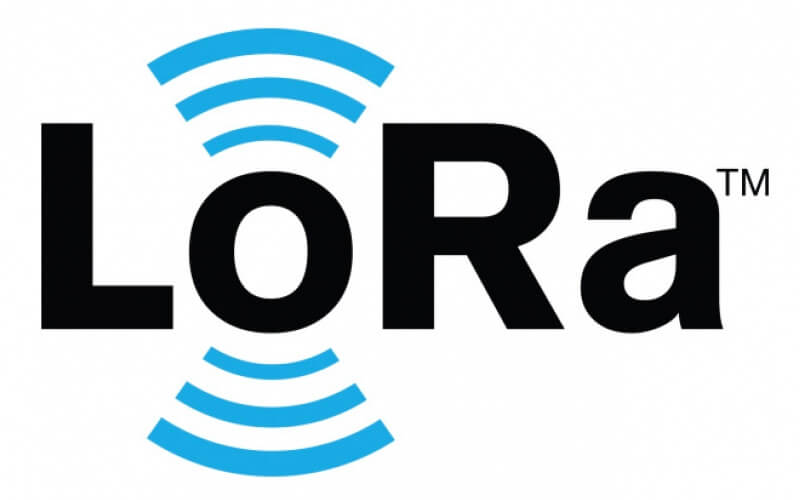
\includegraphics[width=0.28\textwidth]{material/lora-logo.jpg}
  \end{center}
  \begin{exampleblock}{}
  \begin{center}
  \Large Inspiriert von der Natur: Fledermäuse, Delfine, Wale, \ldots
  \end{center}
  \end{exampleblock}
  \begin{itemize}
\item Ist eine proprietäre \alert{Low-Power-Modulationstechnik}, \alert{2014} patentiert von der \href{https://www.semtech.com/lora}{\alert{Semtech Corporation}}.
\item Nutzt die \alert{weltweit} lizenzfreien \alert{ISM}-Funkbänder (Industrial, Scientific and Medical).
  \end{itemize}
  \begin{description}[World record]
    \item[Reichweite] Typischerweise \alert{\SI{10}{\kilo\meter}} mit einem \alert{\SI{25}{\milli\watt}}-Sender.
    \item[\href{https://www.thethingsnetwork.org/article/new-lora-world-record-1336-km-830-mi\#:~:text=The\%20long\%20term\%20LoRaWAN\%C2\%AE,at\%201336\%20km\%20\%2F\%20830\%20miles.}{Weltrekord}] \alert{\SI{1336}{\kilo\meter}} mit einem \SI{25}{\milli\watt}-Sender.
  \end{description}
\end{frame}
